\section{Preliminaries}

Throughout this paper, we assume that the data is generated from a linear model, that is,
\[
  y_i = \beta_0^* + \vec x_i^\T \vec\beta^* + \varepsilon_i \quad\text{for}\quad i \in \{1, 2, \dots, n\},
\]
where we use \(\beta_0^*\) and \(\vec\beta^*\) to denote the true intercept and coefficients, respectively, and \(\varepsilon_i\) to denote measurement noise. \(\mat X\) is the \(n \times p\) design matrix with columns \(\vec x_j\) and \(\vec y\) the \(n \times 1\) response vector.
Furthermore, we use \(\hat\beta_0\) and \(\hat{\vec{\beta}}\) to denote our estimates of the intercept and coefficients and use \(\beta_0\) and \(\beta\) to refer to corresponding variables in the optimization problem.
Unless otherwise stated, we assume \(\mat{X}\), \(\beta_0^*\), and \(\vec{\beta}^*\) to be fixed.

There is ambiguity regarding many of the key terms in the field of normalization. \emph{Scaling}, \emph{standardization}, and \emph{normalizaton} are for instance used interchangeably throughout the literature. Here, we define \emph{normalization} as the process of centering and scaling the feature matrix, which we formalize in \Cref{def:normalization}.

\begin{definition}[Normalization]
  \label{def:normalization}
  % Let \(\mat S\) be the \emph{scaling matrix}, which is a \(p \times p\) diagonal matrix with entries \(s_1, s_2, \dots, s_p\). Let \(\mat C\) be the \emph{centering matrix}, which is an \(n \times p\) matrix with each row equal to \([c_1, c_2, c_n]^\T\). Then the \emph{normalized design matrix} \(\tilde{\mat X}\) is defined as \(\tilde{\mat X} = (\mat X - \mat C)\mat S^{-1}\).
  Let \(\tilde{\mat X}\) be the normalized feature matrix, with
  elements
  \[
    \tilde{x}_{ij} = \frac{x_{ij} - c_{j}}{s_j},
  \]
  where \(x_{ij}\) is an element of the (unnormalized) feature matrix \(\mat{X}\)
  and \(c_j\) and \(s_j\) are the \emph{centering} and \emph{scaling} factors respectively.
\end{definition}

Some authors refer to this procedure as \emph{standardization}, but here we define standardization only as the case when centering with the arithmetic mean and scaling with the (uncorrected) standard deviation. Also note that normalization is sometimes defined as the process of scaling the \emph{samples}, rather than the features. We will not consider this type of normalization in this paper.

\subsection{Types of Normalization}

There are many different strategies for normalizing the design matrix.
We list a few of the most common choices in \Cref{tab:normalization-types}.
In the following sections, we will discuss some basic properties of these normalization strategies that will be useful in subsequent sections of the paper.

\begin{table}[hbt]
  \centering
  \caption{Common ways to normalize a matrix of features}
  \label{tab:normalization-types}
  \begin{tabular}{lll}
    \toprule
    Normalization    & Centering (\(c_{j}\))              & Scaling (\(s_j\))                                         \\
    \midrule
    Standardization  & \(\frac{1}{n}\sum_{i=1}^n x_{ij}\) & \(\sqrt{\frac{1}{n}\sum_{i=1}^n (x_{ij} - \bar{x}_j)^2}\) \\
    \addlinespace
    Min--Max         & \(\min_i(x_{ij})\)                 & \(\max_i(x_{ij}) - \min_i(x_{ij})\)                       \\
    \addlinespace
    Unit Vector (L2) & 0                                  & \(\sqrt{\sum_{i=1}^n x_{ij}^2}\)                          \\
    \addlinespace
    Max--Abs         & 0                                  & \(\max_i(|x_{ij}|)\)                                      \\
    \addlinespace
    Adaptive Lasso   & 0                                  & \(\beta_j^\text{OLS}\)                                    \\
    \bottomrule
  \end{tabular}
\end{table}

\subsubsection{Standardization}

Standardization is perhaps the most common type of normalization, at least in the field of statistics. It is also sometimes known as \emph{z-scoring} or \emph{z-transformation}. One of the benefits of using standardization is that it simplifies certain aspects of fitting the model. For instance, the intercept term \(\hat\beta_0\) is equal to the mean of the response \(\vec y\).

For regularized methods, it is typically the case that we standardize with the uncorrected sample standard deviation (division by \(n\)).

The downside of standardization is that it involves centering by the mean, which typically destroys sparsity in the data structure. This is not a problem when the data is stored as a dense matrix, but when the data is sparse, this can lead to a significant increase in memory usage and computational time.

\subsubsection{Maximum Absolute Value Scaling}

A common alternative to standardization is to scale the features by their maximum absolute value. This is sometimes called \emph{max--abs} scaling. This type of scaling typically has no impact on binary data (since the maximum absolute value is usually 1), and therefore retains sparsity. For other types of data, it scales the features to take values in the range \([-1, 1]\).
This type of scaling is naturally sensitive to outliers, since they will single-handedly determine the scaling factor.

For many types of continuous data, such as normally distributed data, the sample maximum, and therefore the level of scaling in the max--abs method, depends on the sample size~\Cref{thm:maxabs-gev}. This, in addition to the sensitivity to outliers, makes maximum absolute value scaling unsuitable for such data. As a result, we will only discuss it in the context of binary features.

\begin{theorem}
  \label{thm:maxabs-gev}
  Let \(X_1, X_2, \dots, X_n\) be a sample of normally distributed random variables, each with mean \(\mu\) and standard deviation \(\sigma\). Then
  \[
    \lim_{n \rightarrow \infty}\Pr\left(\max_{i \in [n]} |X_i| \leq x\right) = G(x),
  \]
  where \(G\) is the cumulative distribution function of a Gumbel distribution with
  parameters
  \[
    b_n = F_Y^{-1}(1 - 1/n)\quad \text{and} \quad a_n = \frac{1}{n f_Y(\mu_n)},
  \]
  where \(f_Y\) and \(F_Y^{-1}\) are the probability distribution function and quantile function, respectively, of a folded normal distribution with mean \(\mu\) and standard deviation \(\sigma\).
\end{theorem}

As a result of \Cref{thm:maxabs-gev}, the limiting distribution of \(\max_{i \in [n]}|X_i|\) has expected value \(b_n + \gamma a_n\), where \(\gamma\) is the Euler-Mascheroni constant. In \Cref{fig:maxabs-gev}, we verify that the limiting distribution agrees well with the empirical distribution in expected value even for small values of \(n\).

In \Cref{fig:maxabs-n} we show the effect of increasing the number of observations, \(n\), in a two-feature lasso model with max-abs normalization applied to both features. The coefficient corresponding to the Normally distributed feature shrinks as the number of observation \(n\) increases. Since the expected value of the Gumbel distribution diverges with \(n\), this means that there's always a large enough \(n\) to make the coefficient zero with high probability.

\begin{figure}[htpb]
  \centering
  \subcaptionbox{Theoretical versus empirical distribution of the maximum absolute value of normally distributed random variables.\label{fig:maxabs-gev}}{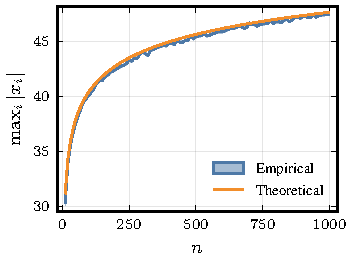
\includegraphics[]{plots/maxabs_gev.pdf}}%
  \hspace{1cm}
  \subcaptionbox{Estimation of mixed features under maximum absolute value scaling\label{fig:maxabs-n}}{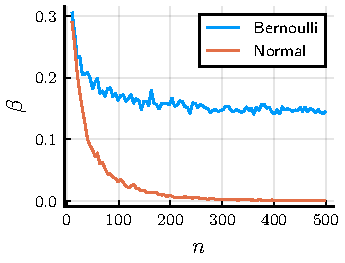
\includegraphics[]{plots/maxabs_n.pdf}}
  \caption{%
    Effects of maximum absolute value scaling.
  }
  \label{fig:maxabs}
\end{figure}

\subsubsection{Min--Max Normalization}

Min-max normalization scales the data to lie in \([0, 1]\). As with maximum absolute value scaling, min-max normalization retains sparsity and also shares its sensitivity to outliers and sample size.

\subsection{The Elastic Net}

From now on, we will direct our focus on the elastic net, which is a combination of the \(\ell_1\) and \(\ell_2\) penalties. The elastic net, for the normalized feature matrix \(\tilde{\mat{X}}\), is represented by the following convex optimization problem:
\begin{equation}
  \label{eq:elastic-net}
  \operatorname*{minimize}_{\beta_0 \in \mathbb{R},\vec{\beta} \in \mathbb{R}^p}\left( L(\beta_0, \vec{\beta};\vec{X},\vec{y},\lambda_1,\lambda_2)=\frac{1}{2} \lVert \vec y - \beta_0 - \tilde{\mat{X}}\vec{\beta} \rVert^2_2  + \lambda_1 \lVert \vec\beta \rVert_1 + \frac{\lambda_2}{2}\lVert \vec \beta \rVert_2^2\right).
\end{equation}
We define \((\hat{\beta}_0^{(n)}, \hat{\vec{\beta}}^{(n)})\) as a solution to the optimization problem in \Cref{eq:elastic-net}.
When \(\lambda_1 > 0\) and \(\lambda_2 = 0\), the elastic net is equivalent to the lasso, and when \(\lambda_1 = 0\) and \(\lambda_2 > 0\), it is equivalent to ridge regression. Expanding \(L\) in \Cref{eq:elastic-net}, we have
\[
  \begin{aligned}
    \frac{1}{2}\left( \vec y^\T \vec y - 2(\tilde{\mat{X}}\vec{\beta} + \beta_0)^\T\vec{y} + (\tilde{\mat{X}}\vec{\beta} + \beta_0)^\T(\tilde{\mat{X}}\vec{\beta} + \beta_0)\right) + \lambda_1 \lVert \vec\beta \rVert_1 + \frac{\lambda_2}{2}\lVert \vec \beta \rVert_2^2.
  \end{aligned}
\]
Taking the subdifferential with respect to \(\vec{\beta}\) and \(\beta_0\), the KKT stationarity condition yields the following system of equations:
\begin{equation}
  \label{eq:kkt-elasticnet}
  \begin{cases}
    \tilde{\mat{X}}^\T(\tilde{\mat{X}}\vec{\beta} + \beta_0 - \vec{y}) + \lambda_1 g + \lambda_2 \vec\beta \ni \vec{0}, \\
    n \beta_0 + (\tilde{\mat{X}}\vec{\beta})^\T \vec{1} - \vec{y}^\T \vec{1} = 0.
  \end{cases}
\end{equation}
Here, \(g\) is a subgradient of the \(\ell_1\) norm, which has elements \(g_i\) such that
\[
  g_i \in
  \begin{cases}
    \{\sign{\beta_i}\} & \text{if } \beta_i \neq 0, \\
    [-1, 1]            & \text{otherwise}.
  \end{cases}
\]

\subsection{Rescaling Regression Coefficients}

Normalization changes the optimization problem and therefore its solution, the coefficients, which will now be on the scale of the normalized features. We, however, are interested in \(\hat{\vec{\beta}}\): the coefficients on the scale of the original problem. To obtain estimates of these, we transform the coefficients from the normalized poblem, \(\hat\beta^{(n)}_j\), back via
\[
  \hat\beta_j = \frac{\hat\beta^{(n)}_j}{s_j} \quad\text{for}\quad j = 1,2,\dots,p.
\]
There is a similar transformation for the intercept which we omit here since we are not interested in interpreting it.

\subsection{Orthogonal Features}

If the features of the normalized design matrix are orthogonal, that is, \(\tilde{\mat{X}}^\intercal \tilde{\mat{X}} = \diag\left(\tilde{\vec{x}}_1^\T \tilde{\vec{x}}_1, \dots, \tilde{\vec{x}}_p^\intercal \tilde{\vec{x}}_p\right) \), then \Cref{eq:kkt-elasticnet} can be decomposed into a set of \(p + 1\) conditions:
\[
  \begin{cases}
    \tilde{\vec{x}}_j^\T \tilde{\vec{x}}_j \beta_j + \tilde{\vec{x}}_j^\T \ones \beta_0 - \tilde{\vec{x}}_j^\T\vec{y} + \lambda_2 \beta_j + \lambda_1 g \ni 0, & j=1,\dots,p, \\
    n \beta_0 + (\tilde{\mat{X}}\vec{\beta})^\T \vec{1} -  \vec{y}^\T \ones = 0.
  \end{cases}
\]
The inclusion of an intercept, \(\beta_0\), ensures that the location of the
features (their means) does not affect the solution (except for the intercept itself). Therefore,
we will from now on assume that the features are mean-centered, that is, \(c_j = \bar{\vec{x}}_j\) for all \(j\) and therefore \(\tilde{\vec{x}}_j^\T \ones = 0\). A solution to the system of equations is then given by the following set of equations~\citep{donoho1994}:
\begin{equation}
  \label{eq:orthogonal-solution}
  \hat\beta_j = \frac{\st_{\lambda_1}\left(\tilde{\vec{x}}_j^\T \vec{y}\right)}{s_j\left(\tilde{\vec{x}}_j^\T \tilde{\vec{x}}_j + \lambda_2\right)},
  \qquad
  \hat\beta_0 = \frac{\vec{y}^\T \ones}{n},
\end{equation}
where \(\st\) is the soft-thresholding operator, defined as
\[
  \st_\lambda(z) = \sign(z) \max(|z| - \lambda, 0) = \ind{|z|>\lambda}\big(z - \sign(z)\lambda\big).
\]
